\chapter{Vista de desarrollo}
Esta vista es fundamental como punto de partida para el equipo de desarrollo para saber como iniciar y organizar el código. El software quedará dividido en varios subsistemas (que a su vez están organizados en capas o jerarquías) que pueden ser desarrollados por uno o varios desarrolladores.

Para poder definir esta vista, previamente se ha tenido que identificar y definir todos los elementos del software.

(Incluir diagrama de paquetes y diagrama de componentes)

\begin{figure}
	\centering
	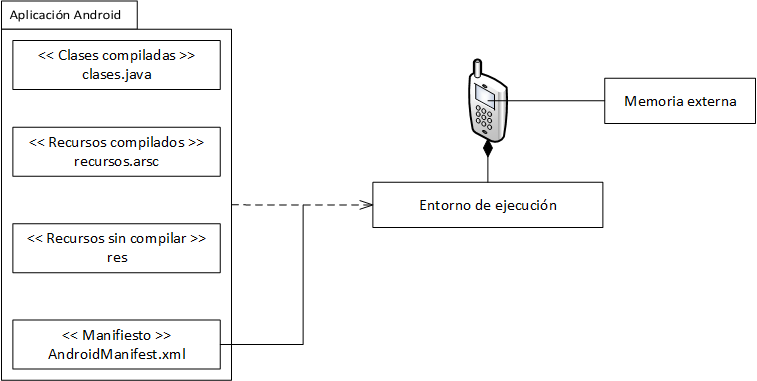
\includegraphics[width=0.65\textwidth]{4.Disenio/Imagenes/AppAndroid}
	\caption{Despliegue de la aplicación Android.}
	\label{fig:appAndroid}
\end{figure}
